\iffalse
This file is protected by Copyright. Please refer to the COPYRIGHT file
distributed with this source distribution.

This file is part of OpenCPI <http://www.opencpi.org>

OpenCPI is free software: you can redistribute it and/or modify it under the
terms of the GNU Lesser General Public License as published by the Free Software
Foundation, either version 3 of the License, or (at your option) any later
version.

OpenCPI is distributed in the hope that it will be useful, but WITHOUT ANY
WARRANTY; without even the implied warranty of MERCHANTABILITY or FITNESS FOR A
PARTICULAR PURPOSE. See the GNU Lesser General Public License for more details.

You should have received a copy of the GNU Lesser General Public License along
with this program. If not, see <http://www.gnu.org/licenses/>.
\fi

%----------------------------------------------------------------------------------------
% Required document specific properties
%----------------------------------------------------------------------------------------
\def\comp{cic\_{}int}
\edef\ecomp{cic_int}
\def\Comp{CIC Interpolator}
\def\docTitle{\Comp{} Component Data Sheet}
\def\snippetpath{../../../../../../doc/av/tex/snippets}
%----------------------------------------------------------------------------------------
% Global latex header (this must be after document specific properties)
%----------------------------------------------------------------------------------------
\iffalse
This file is protected by Copyright. Please refer to the COPYRIGHT file
distributed with this source distribution.

This file is part of OpenCPI <http://www.opencpi.org>

OpenCPI is free software: you can redistribute it and/or modify it under the
terms of the GNU Lesser General Public License as published by the Free Software
Foundation, either version 3 of the License, or (at your option) any later
version.

OpenCPI is distributed in the hope that it will be useful, but WITHOUT ANY
WARRANTY; without even the implied warranty of MERCHANTABILITY or FITNESS FOR A
PARTICULAR PURPOSE. See the GNU Lesser General Public License for more details.

You should have received a copy of the GNU Lesser General Public License along
with this program. If not, see <http://www.gnu.org/licenses/>.
\fi

% Sets OpenCPI Version used throughout all the docs. This is updated by
% scripts/update-release.sh when a release is being made and must not
% be changed manually.
\def\ocpiversion{v2.2.0}

\documentclass{article}
\author{}  % Force author to be blank
\date{OpenCPI Release:\ \ \ocpiversion}  % Force date to be blank and override date with version
\title{OpenCPI\\\docTitle}  % docTitle must be defined before including this file
%----------------------------------------------------------------------------------------
% Paper size, orientation and margins
%----------------------------------------------------------------------------------------
\usepackage{geometry}
\geometry{
  letterpaper,  % paper type
  portrait,     % text direction
  left=.75in,   % left margin
  top=.75in,    % top margin
  right=.75in,  % right margin
  bottom=.75in  % bottom margin
}
%----------------------------------------------------------------------------------------
% Header/Footer
%----------------------------------------------------------------------------------------
\usepackage{fancyhdr} \pagestyle{fancy}  % required for fancy headers
\renewcommand{\headrulewidth}{0.5pt}
\renewcommand{\footrulewidth}{0.5pt}
\lhead{\small{\docTitle}}
\rhead{\small{OpenCPI}}
%----------------------------------------------------------------------------------------
% Various packages
%----------------------------------------------------------------------------------------
\usepackage{amsmath}
\usepackage[page,toc]{appendix}  % for appendix stuff
\usepackage{enumitem}
\usepackage{graphicx}   % for including pictures by file
\usepackage{hyperref}   % for linking urls and lists
\usepackage{listings}   % for coding language styles
\usepackage{pdflscape}  % for landscape view
\usepackage{pifont}     % for sideways table
\usepackage{ragged2e}   % for justify
\usepackage{rotating}   % for sideways table
\usepackage{scrextend}
\usepackage{setspace}
\usepackage{subfig}
\usepackage{textcomp}
\usepackage[dvipsnames,usenames]{xcolor}  % for color names see https://en.wikibooks.org/wiki/LaTeX/Colors
\usepackage{xstring}
\uchyph=0  % Never hyphenate acronyms like RCC
\renewcommand\_{\textunderscore\allowbreak}  % Allow words to break/newline on underscores
%----------------------------------------------------------------------------------------
% Table packages
%----------------------------------------------------------------------------------------
\usepackage[tableposition=top]{caption}
\usepackage{float}
\floatstyle{plaintop}
\usepackage{longtable}  % for long possibly multi-page tables
\usepackage{multicol}   % for more advanced table layout
\usepackage{multirow}   % for more advanced table layout
\usepackage{tabularx}   % c=center,l=left,r=right,X=fill
% These define tabularx columns "C" and "R" to match "X" but center/right aligned
\newcolumntype{C}{>{\centering\arraybackslash}X}
\newcolumntype{M}[1]{>{\centering\arraybackslash}m{#1}}
\newcolumntype{P}[1]{>{\centering\arraybackslash}p{#1}}
\newcolumntype{R}{>{\raggedleft\arraybackslash}X}
%----------------------------------------------------------------------------------------
% Block Diagram / FSM Drawings
%----------------------------------------------------------------------------------------
\usepackage{tikz}
\usetikzlibrary{arrows,decorations.markings,fit,positioning,shapes}
\usetikzlibrary{automata}  % used for the fsm
\usetikzlibrary{calc}      % for duplicating clients
\usepgfmodule{oo}          % to define a client box
%----------------------------------------------------------------------------------------
% Colors Used
%----------------------------------------------------------------------------------------
\usepackage{colortbl}
\definecolor{blue}{rgb}{.7,.8,.9}
\definecolor{ceruleanblue}{rgb}{0.16, 0.32, 0.75}
\definecolor{cyan}{rgb}{0.0,0.6,0.6}
\definecolor{darkgreen}{rgb}{0,0.6,0}
\definecolor{deepmagenta}{rgb}{0.8, 0.0, 0.8}
\definecolor{maroon}{rgb}{0.5,0,0}
%----------------------------------------------------------------------------------------
% Define where to hyphenate
%----------------------------------------------------------------------------------------
\hyphenation{Cent-OS}
\hyphenation{install-ation}
%----------------------------------------------------------------------------------------
% Define Commands & Rename Commands
%----------------------------------------------------------------------------------------
\newcommand{\code}[1]{\texttt{#1}}  % For inline code snippet or command line
\newcommand{\sref}[1]{Section~\ref{#1}}  % To quickly reference a section
\newcommand{\todo}[1]{\textcolor{red}{TODO: #1}\PackageWarning{TODO:}{#1}}  % To do notes
\renewcommand{\contentsname}{Table of Contents}
\renewcommand{\listfigurename}{List of Figures}
\renewcommand{\listtablename}{List of Tables}

% This gives a link to gitlab.io document. By default, it outputs the filename.
% You can optionally change the link, e.g.
% \githubio{FPGA\_Vendor\_Tools\_Installation\_Guide.pdf} vs.
% \githubio[\textit{FPGA Vendor Tools Installation Guide}]{FPGA\_Vendor\_Tools\_Installation\_Guide.pdf}
% or if you want the raw ugly URL to come out, \githubioURL{FPGA_Vendor_Tools_Installation_Guide.pdf}
\newcommand{\githubio}[2][]{% The default is for FIRST param!
\href{http://opencpi.gitlab.io/releases/\ocpiversion/docs/#2}{\ifthenelse{\equal{#1}{}}{\texttt{#2}}{#1}}}
\newcommand{\gitlabcom}[2][]{% The default is for FIRST param!
\href{http://gitlab.com/opencpi/#2}{\ifthenelse{\equal{#1}{}}{\texttt{#2}}{#1}}}
\newcommand{\githubioURL}[1]{\url{http://opencpi.gitlab.io/releases/\ocpiversion/docs/#1}}
% Lastly, if you want a SINGLE leading path stripped, e.g. assets/X.pdf => X.pdf:
\newcommand{\githubioFlat}[1]{%
\StrBehind{#1}{/}[\den]%
\href{http://opencpi.gitlab.io/releases/\ocpiversion/docs/#1}{\texttt{\den}}%
}
%----------------------------------------------------------------------------------------
% VHDL Coding Language Style
% modified from: http://latex-community.org/forum/viewtopic.php?f=44&t=22076
%----------------------------------------------------------------------------------------
\lstdefinelanguage{VHDL}
{
  basicstyle=\ttfamily\footnotesize,
  columns=fullflexible,keepspaces,  % https://tex.stackexchange.com/a/46695/87531
  keywordstyle=\color{ceruleanblue},
  commentstyle=\color{darkgreen},
  morekeywords={
    library, use, all, entity, is, port, in, out, end, architecture, of,
    begin, and, signal, when, if, else, process, end,
  },
  morecomment=[l]--
}
%----------------------------------------------------------------------------------------
% XML Coding Language Style
% modified from http://tex.stackexchange.com/questions/10255/xml-syntax-highlighting
%----------------------------------------------------------------------------------------
\lstdefinelanguage{XML}
{
  basicstyle=\ttfamily\footnotesize,
  columns=fullflexible,keepspaces,
  morestring=[s]{"}{"},
  morecomment=[s]{!--}{--},
  commentstyle=\color{darkgreen},
  moredelim=[s][\color{black}]{>}{<},
  moredelim=[s][\color{cyan}]{\ }{=},
  stringstyle=\color{maroon},
  identifierstyle=\color{ceruleanblue}
}
%----------------------------------------------------------------------------------------
% DIFF Coding Language Style
% modified from http://tex.stackexchange.com/questions/50176/highlighting-a-diff-file
%----------------------------------------------------------------------------------------
\lstdefinelanguage{diff}
{
  basicstyle=\ttfamily\footnotesize,
  columns=fullflexible,keepspaces,
  breaklines=true,                            % wrap text
  morecomment=[f][\color{ceruleanblue}]{@@},  % group identifier
  morecomment=[f][\color{red}]-,              % deleted lines
  morecomment=[f][\color{darkgreen}]+,        % added lines
  morecomment=[f][\color{deepmagenta}]{---},  % Diff header lines (must appear after +,-)
  morecomment=[f][\color{deepmagenta}]{+++},
}
%----------------------------------------------------------------------------------------
% Python Coding Language Style
%----------------------------------------------------------------------------------------
\lstdefinelanguage{python}
{
  basicstyle=\ttfamily\footnotesize,
  columns=fullflexible,keepspaces,
  keywordstyle=\color{ceruleanblue},
  commentstyle=\color{darkgreen},
  stringstyle=\color{orange},
  morekeywords={
    print, if, sys, len, from, import, as, open,close, def, main, for, else,
    write, read, range,
  },
  comment=[l]{\#}
}
%----------------------------------------------------------------------------------------
% Fontsize Notes in order from smallest to largest
%----------------------------------------------------------------------------------------
%    \tiny
%    \scriptsize
%    \footnotesize
%    \small
%    \normalsize
%    \large
%    \Large
%    \LARGE
%    \huge
%    \Huge

\def\importpath{../../cic_dec.test/doc/}  % Reuse existing content for CIC Decimator
\graphicspath{{figures/}}
%----------------------------------------------------------------------------------------

\begin{document}
\maketitle
\thispagestyle{empty}
\newpage

\def\name{\comp}
\def\workertype{Application}
\def\version{\ocpiversion}
\def\releasedate{4/2019}
\def\componentlibrary{ocpi.assets.dsp\_{}comps}
\def\workers{\comp{}.hdl}
\def\testedplatforms{alst4, isim, Matchstiq-Z1(PL), ml605, modelsim, xsim, ZedBoard(PL)}
\section*{Summary - \Comp}
\begin{tabular}{|c|M{13.5cm}|}
  \hline
  \rowcolor{blue}
   & \\
  \hline
  Name              & \comp             \\
  \hline
  Worker Type       & \workertype       \\
  \hline
  OpenCPI Release   & \ocpiversion      \\
  \hline
  Last Update       & \releasedate      \\
  \hline
  Component Library & \componentlibrary \\
  \hline
  Workers           & \workers          \\
  \hline
  Tested Platforms  & \testedplatforms  \\
  \hline
\end{tabular}


\section*{Functionality}
\begin{flushleft}
	The CIC interpolator has \verb+N+ cascaded comb stages with an input data rate of $\frac{f_{s}}{R}$, followed by a rate change by a factor \verb+R+, followed by \verb+N+ cascaded integrator stages with an output data rate of $f_{s}$. The differential delay, \verb+M+, affects the slope of the transition region. Figure \ref{fig:cic} diagrams the interpolating CIC filter.

	\begin{figure}[ht]
		\centering
		\includegraphics[scale=.6]{cic_interpolator_block_diagram}
		\caption{Cascaded Integration Comb Decimation filter Block Diagram}
		\label{fig:cic}
	\end{figure}
\end{flushleft}

\section*{Worker Implementation Details}
\input{\importpath snippets/CIC_HDL_Implementation}
\input{\importpath snippets/CIC_Theory}

\section*{Block Diagrams}
\subsection*{Top level}
\begin{center}
	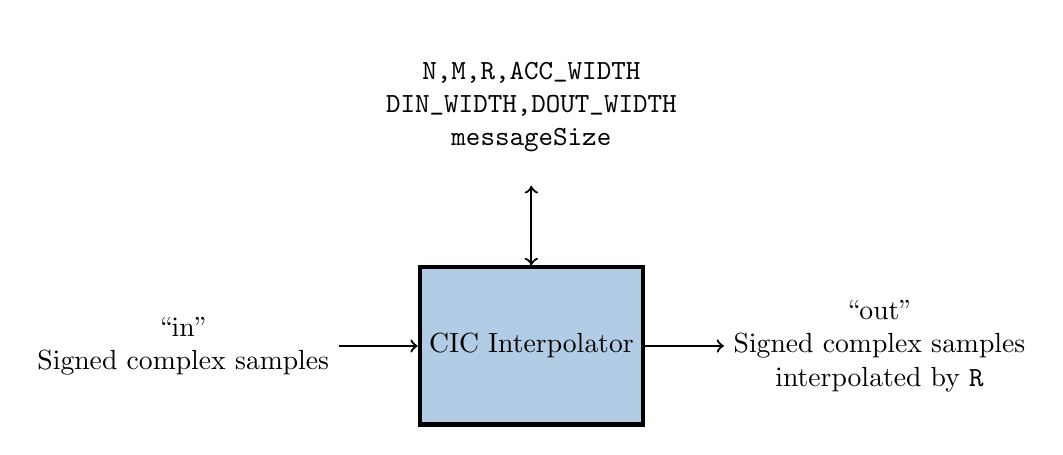
\begin{tikzpicture}[% List of styles applied to all, to override specify on a case-by-case
			every node/.style={
				align=center,  		% use this so that the "\\" for line break works
				minimum size=2cm	% creates space above and below text in rectangle
			},
			every edge/.style={draw,thick}
		]
		\node[rectangle,ultra thick,draw=black,fill=blue](R2){\Comp};
		\node[rectangle,draw=white,fill=white](R3)[left= of R2]{``in'' \\ Signed complex samples};
		\node[rectangle,draw=white,fill=white](R4)[right= of R2]{``out'' \\ Signed complex samples \\ interpolated by \verb+R+};
		\node[rectangle,draw=white,fill=white](R5)[above= of R2]{\verb+N,M,R,ACC_WIDTH+ \\ \verb+DIN_WIDTH,DOUT_WIDTH+ \\ \verb+messageSize+};
		\path[->]
		(R3)edge []	node [] {} (R2)
		(R2)edge []	node [] {} (R4)
		(R2)edge []	node [] {} (R5)
		(R5)edge []	node [] {} (R2)
		;
	\end{tikzpicture}
	\captionof{figure}{Top Level Block Diagram}
\end{center}
\newpage

\section*{Source Dependencies}
\subsection*{\comp.hdl}
\begin{itemize}
	\item assets/components/dsp\_comps/cic\_int.hdl/cic\_int.vhd
	\item assets/hdl/primitives/dsp\_prims/dsp\_prims\_pkg.vhd
	      \subitem assets/hdl/primitives/dsp\_prims/cic/src/cic\_int\_gen.vhd
\end{itemize}

\begin{landscape}
	\section*{Component Spec Properties}
	\begin{scriptsize}
		\begin{tabular}{|p{3cm}|p{1.5cm}|c|c|c|c|c|p{7cm}|}
			\hline
			\rowcolor{blue}
			Name                      & Type   & SequenceLength & ArrayDimensions & Accessibility      & Valid Range & Default & Usage                                            \\
			\hline \verb+N+           & UChar  & -              & -               & Readable           & -           & -       & Number of Stages                                 \\
			\hline \verb+M+           & UChar  & -              & -               & Readable           & -           & -       & Differential Delay                               \\
			\hline \verb+R+           & UShort & -              & -               & Readable           & -           & -       & Interpolation Factor                             \\
			\hline \verb+ACC_WIDTH+   & UChar  & -              & -               & Readable           & -           & -       & Accumulation Width *(\ref{eq:response_function}) \\
			\hline \verb+DIN_WIDTH+   & UChar  & -              & -               & Readable           & -           & -       & Input data width                                 \\
			\hline \verb+DOUT_WIDTH+  & UChar  & -              & -               & Readable           & -           & -       & Output data width                                \\
			\hline \verb+messageSize+ & UShort & -              & -               & Readable, Writable & -           & 8192    & Number of bytes in output message                \\
			\hline
		\end{tabular}
	\end{scriptsize}
	\section*{Worker Properties}

	\subsection*{\comp.hdl}
	\begin{scriptsize}
		\begin{tabular}{|c|p{2cm}|p{1cm}|c|c|c|p{2cm}|p{1cm}|p{5cm}|}
			\hline
			\rowcolor{blue}
			Type         & Name              & Type & SequenceLength & ArrayDimensions & Accessibility & Valid Range & Default & Usage                                            \\
			\hline
			SpecProperty & \verb+N+          & -    & -              & -               & Parameter     & 3-6         & 3       & Number of Stages                                 \\
			\hline
			SpecProperty & \verb+M+          & -    & -              & -               & Parameter     & 1-2         & 1       & Differential Delay                               \\
			\hline
			SpecProperty & \verb+R+          & -    & -              & -               & Parameter     & 4-8192      & 4       & Decimation Factor                                \\
			\hline
			SpecProperty & \verb+DIN_WIDTH+  & -    & -              & -               & Parameter     & 16          & 16      & Input Data Width                                 \\
			\hline
			SpecProperty & \verb+ACC_WIDTH+  & -    & -              & -               & Parameter     & *           & 22      & Accumulation Width *(\ref{eq:response_function}) \\
			\hline
			SpecProperty & \verb+DOUT_WIDTH+  & -    & -              & -               & Parameter           & 16          & 16      & Output Data Width                                \\
			\hline
			Property     & \verb+CHIPSCOPE_p+ & Bool & -              & -               & Readable, Parameter & Standard    & false   & Include ISE ChipScope circuit                        \\
			\hline
			Property     & \verb+VIVADO_ILA_p+ & Bool & -              & -               & Readable, Parameter & Standard    & false   & Include Vivado Integrated Logic Analyzer circuit                        \\
			\hline
		\end{tabular}
	\end{scriptsize}

	\section*{Component Ports}
	\begin{scriptsize}
		\begin{tabular}{|p{2cm}|p{1.5cm}|p{4cm}|p{1.5cm}|p{1.5cm}|p{10.75cm}|}
			\hline
			\rowcolor{blue}
			Name & Producer & Protocol           & Optional & Advanced & Usage                  \\
			\hline
			in   & False    & iqstream\_protocol & False     & -        & Complex signed samples (Q0.15 I, Q0.15 Q). \\
			\hline
			out  & False    & iqstream\_protocol & False     & -        & Complex signed samples (Q0.15 I, Q0.15 Q). \\
			\hline
		\end{tabular}
	\end{scriptsize}

	\section*{Worker Interfaces}
	\subsection*{\comp.hdl}
	\begin{scriptsize}
		\begin{tabular}{|M{2cm}|M{1.5cm}|c|c|M{12cm}|}
			\hline
			\rowcolor{blue}
			Type            & Name & DataWidth & Advanced                & Usage                  \\
			\hline
			StreamInterface & in   & 32        & ZeroLengthMessages=true & Signed complex samples \\
			\hline
			StreamInterface & out  & 32        & ZeroLengthMessages=true & Signed complex samples \\
			\hline
		\end{tabular}
	\end{scriptsize}
\end{landscape}

\section*{Control Timing and Signals}
\begin{flushleft}
	The CIC Interpolation filter HDL worker uses the clock from the Control Plane and standard Control Plane signals.\medskip

	%\noindent This worker has an processing group delay of (N*R*M + R*2 + 2) valid input data cycles. After this initial delay, valid output data is given N*2+1 clock cycles after input data is taken.\par\bigskip

	This worker has a latency of \verb+N+*2+1 valid input data clock cycles.\medskip

	\begin{tabular}{|M{4.5cm}|M{4.5cm}|M{1cm}|M{1.5cm}|M{2cm}|M{1cm}|M{1cm}|M{2.5cm}|}
		\hline
		\rowcolor{blue}
		\hline
		Latency         \\
		\hline
		\verb+N+*2+1    \\
		\hline
	\end{tabular}
\end{flushleft}

\begin{landscape}
\section*{Worker Configuration Parameters}
\subsubsection*{\comp.hdl}
%\input{../../\ecomp.hdl/configurations.inc}
\section*{Performance and Resource Utilization}
\subsection*{\comp.hdl}
%\input{../../\ecomp.hdl/utilization.inc}
\end{landscape}
\newpage
\section*{Test and Verification}
Two test cases are implemented to validate the CIC Interpolator component:

\begin{enumerate}
	\item Unity gain response to DC: The CIC Interpolator gain is calculated using the following equation:
	      \begin{equation} \label{eq:cic_gain}
	      	CIC\ Gain = \frac{(R*M)^N}{2^{CEIL(N*log_2(R*M))}}
	      \end{equation}
	\item Tone waveform: A waveform containing a tone at 50 Hz is sampled at 1024000/R and processed by the worker. The output data (interpolated waveform) is checked to ensure the 50 Hz tone is present.
\end{enumerate}\medskip

For the plots below, a CIC Interpolator with the following parameter set was used: \verb+N+=3, \verb+M+=1, \verb+R+=2048, and \verb+ACC_WIDTH+=49.\bigskip

\newpage
	For Case \#1, the plots below show the input with the I-leg zoomed in the show the amplitude is 32767, and output data with the I-leg zoomed to show an amplitude of 32767, which can be calculated using \ref{eq:cic_gain}, shown below, and the Q-leg showing the worker delay before reaching it steady-state value.
		  \begin{equation} \label{eq:cic_gain_applied}
	      	Output Amplitude = 32767*\frac{(2048*1)^3}{2^{CEIL(3*log_2(2038*1))}} = 32767*1=32767
	      \end{equation}

	\begin{figure}[ht]
		\centering
		\begin{minipage}{.5\textwidth}
			\centering\includegraphics[width=1.0\linewidth]{input_time_DC}
			\captionof{figure}{Time Domain: DC with amp=32767}
			\label{fig:input_time_DC}
		\end{minipage}%
		\begin{minipage}{.5\textwidth}
			\centering\includegraphics[width=1.0\linewidth]{input_freq_DC}
			\captionof{figure}{Frequency Domain: 0 Hz}
			\label{fig:input_freq_DC}
		\end{minipage}
	\end{figure}


	\begin{figure}[ht]
		\centering
		\begin{minipage}{.5\textwidth}
			\centering\includegraphics[width=1.0\linewidth]{output_time_DC}
			\captionof{figure}{Time Domain: DC with amp=32767}
			\label{fig:output_time_DC}
		\end{minipage}%
		\begin{minipage}{.5\textwidth}
			\centering\includegraphics[width=1.0\linewidth]{output_freq_DC}
			\captionof{figure}{Frequency Domain: 0 Hz}
			\label{fig:output_freq_DC}
		\end{minipage}
	\end{figure}

\newpage
The input time-domain plot below shows the I-leg zoomed into one cycle and Q-leg showing all samples of a 50 Hz tone sampled at 1024000/R=1024000/2048=500 Hz, which results in 10 samples/cycle. The input freq-domain plot shows the generated tone at 50 Hz.
The output time-domain plot below shows the I-leg zoomed into approximately two cycles and Q-leg showing all samples of a 50 Hz tone sampled at (1024000/R)*R=(1024000/2048)*2048=1024000 Hz, which results in 20480 samples/cycle. The output freq-domain plot shows the expected tone at 50 Hz.

	\begin{figure}[ht]
		\centering
		\begin{minipage}{.5\textwidth}
			\centering\includegraphics[width=1.0\linewidth]{input_time_R2048}
			\captionof{figure}{Time Domain}
			\label{fig:input_time_R2048}
		\end{minipage}%
		\begin{minipage}{.5\textwidth}
			\centering\includegraphics[width=1.0\linewidth]{input_freq_R2048}
			\captionof{figure}{Frequency Domain: 50 Hz}
			\label{fig:input_freq_R2048}
		\end{minipage}
	\end{figure}

	\begin{figure}[ht]
		\centering
		\begin{minipage}{.5\textwidth}
			\centering\includegraphics[width=1.0\linewidth]{output_time_R2048}
			\captionof{figure}{Time Domain}
			\label{fig:output_time_R2048}
		\end{minipage}%
		\begin{minipage}{.5\textwidth}
			\centering\includegraphics[width=1.0\linewidth]{output_freq_R2048}
			\captionof{figure}{Frequency Domain: 50 Hz}
			\label{fig:output_freq_R2048}
		\end{minipage}
	\end{figure}

\input{\importpath snippets/CIC_References}

\end{document}
